\documentclass[10pt,conference]{IEEEtran}

\usepackage{url}
\usepackage{amsmath, amssymb}
\usepackage{natbib}
\usepackage{kotex}
\usepackage[T1]{fontenc}
\usepackage{beramono}
\usepackage{listings}
\usepackage{xcolor}
\usepackage{qtree}
\usepackage{multirow}
\usepackage{colortbl}
\usepackage{ulem}
\usepackage{graphicx}
\usepackage{caption}
\usepackage{subcaption}
\usepackage{listings}
\usepackage{enumitem}
\usepackage{algorithm}
\usepackage[noend]{algpseudocode}
\usepackage{booktabs}
\usepackage{makecell}

% load macros
% names
\newcommand{\cfg}{\text{CFG}}
\newcommand{\bnf}{\text{BNF}}
\newcommand{\es}{\text{ES}}
\newcommand{\bnfes}{\bnf_\es}
\newcommand{\peg}{\text{PEG}}

% codes
\newcommand{\scode}[1]{\texttt{\scriptsize#1}}
\newcommand{\code}[1]{\texttt{\footnotesize#1}}
\newcommand{\kwtrue}{\code{true}}
\newcommand{\kwt}{\code{\#t}}
\newcommand{\kwfalse}{\code{false}}
\newcommand{\kwf}{\code{\#f}}

%BNF_ES
\newcommand{\symb}{s}
\newcommand{\NT}[1]{#1}
\newcommand{\T}[1]{\code{#1}}
\newcommand{\argument}{a}
\newcommand{\param}{p}
\newcommand{\butnot}{\!\smallsetminus\!}
\newcommand{\rhs}{\alpha}
\newcommand{\cond}{c}
\newcommand{\nolt}{\left<\neg\code{LT}\right>}

% colors
\newcommand{\inred}[1]{{\color{red}{#1}}}

% lookahead
\newcommand{\symbfirst}[1]{\textbf{first}_\symb(#1)}
\newcommand{\rhsfirst}[1]{\textbf{first}_\rhs(#1)}
\newcommand{\fail}{FAIL}
\newcommand{\emptyfirst}{\circ}
\newcommand{\firstplus}{:\!\!+\;}
\newcommand{\la}{L}
\newcommand{\getlap}[1]{\textbf{get}_\symb(#1)}

% IR_ES language
\newcommand{\ires}{\text{IR}_\text{ES}}
\newcommand{\tend}{\downarrow}
\newcommand{\tin}{\searrow}
\newcommand{\tout}{\swarrow}
\newcommand{\tstar}{\star}

% hint image
\newcommand{\hint}{%
  \begingroup\normalfont
  \includegraphics[height=\fontcharht\font`\B]{img/hint.png}%
  \endgroup
}

% Our tool name
\newcommand{\tool}{\text{\sf JSECT}}
\newcommand{\jiset}{\text{\sf JISET}}

% K framework
\newcommand{\kframework}{\mathbb{K}}

% IRES
\newcommand{\irinst}{i}
\newcommand{\irexpr}{e}
\newcommand{\irvalue}{v}
\newcommand{\irstate}{\sigma}

% Scala code style
\definecolor{dkgreen}{rgb}{0,0.6,0}
\definecolor{gray}{rgb}{0.5,0.5,0.5}
\definecolor{mauve}{rgb}{0.58,0,0.82}
\lstdefinestyle{myScalastyle}{
  frame=tb,
  language=scala,
  aboveskip=3mm,
  belowskip=3mm,
  showstringspaces=false,
  columns=fixed,
  basicstyle={\footnotesize\ttfamily},
  numbers=none,
  keywordstyle=\color{blue},
  commentstyle=\color{dkgreen},
  stringstyle=\color{mauve},
  frame=single,
  breaklines=true,
  breakatwhitespace=true,
  tabsize=3,
}
\lstdefinestyle{smallScalastyle}{
  frame=tb,
  language=scala,
  aboveskip=3mm,
  belowskip=3mm,
  showstringspaces=false,
  columns=fixed,
  basicstyle={\scriptsize\ttfamily},
  numbers=none,
  keywordstyle=\color{blue},
  commentstyle=\color{dkgreen},
  stringstyle=\color{mauve},
  frame=single,
  breaklines=true,
  breakatwhitespace=true,
  tabsize=3,
}

% ECMAScript Intermediate Reprentations
\lstdefinestyle{ires}{
  frame=tb,
  aboveskip=3mm,
  belowskip=3mm,
  showstringspaces=false,
  columns=fixed,
  basicstyle={\footnotesize\ttfamily},
  numbers=none,
  keywordstyle=\color{blue},
  commentstyle=\color{dkgreen},
  stringstyle=\color{mauve},
  frame=single,
  breaklines=true,
  breakatwhitespace=true,
  tabsize=3,
}

% JavaScript code style
\lstdefinelanguage{JavaScript}{
  keywords={typeof, new, true, false, catch, function, return, null, catch, switch, var, if, in, while, do, else, case, break},
  keywordstyle=\color{blue}\bfseries,
  ndkeywords={class, export, boolean, throw, implements, import, this},
  ndkeywordstyle=\color{darkgray}\bfseries,
  identifierstyle=\color{black},
  sensitive=false,
  comment=[l]{//},
  morecomment=[s]{/*}{*/},
  commentstyle=\color{purple}\ttfamily,
  stringstyle=\color{red}\ttfamily,
  morestring=[b]',
  morestring=[b]"
}

\lstdefinestyle{myJSstyle}{
  language=JavaScript,
  extendedchars=true,
  basicstyle=\footnotesize\ttfamily,
  showstringspaces=false,
  showspaces=false,
  numbers=none,
  tabsize=2,
  breaklines=true,
  showtabs=false,
  captionpos=b
}


\begin{document}

\title{N+1 Version Testing for ECMAScript with JavaScript Engines}


\author{
  \IEEEauthorblockN{Jihyeok Park}
  \IEEEauthorblockA{\textit{School of Computing} \\
  \textit{KAIST}\\
  Daejeon, South Korea\\
  jhpark0223@kaist.ac.kr}

  \and

  \IEEEauthorblockN{Seungmin An}
  \IEEEauthorblockA{\textit{School of Computing} \\
  \textit{KAIST}\\
  Daejeon, South Korea\\
  h2oche@kaist.ac.kr}

  \and

  \IEEEauthorblockN{Gyeongwon Kim}
  \IEEEauthorblockA{\textit{School of Computing} \\
  \textit{KAIST}\\
  Daejeon, South Korea\\
  sutt69@kaist.ac.kr}

  \and

  \IEEEauthorblockN{Sukyoung Ryu}
  \IEEEauthorblockA{\textit{School of Computing} \\
  \textit{KAIST}\\
  Daejeon, South Korea\\
  sryu.cs@kaist.ac.kr}
}

\maketitle

\begin{abstract}
  Modern programming follows the continuous integration (CI) and continuous
  deployment (CD) approach rather than the traditional waterfall model.  Even
  the development of modern programming languages uses the CI/CD approach to
  swiftly provide new language features and to adapt new development
  environments.  Unlike the conventional approaches, in the modern CI/CD
  approaches, the language specification is no more the Oracle of semantics
  because both the specification and interpreters (or compilers) can co-evolve.
  In this setting, both the specification and implementations may have bugs, and
  guaranteeing their correctness is non-trivial.

  In this paper, we present a novel \textit{$N$+1-version testing} to resolve
  the problem.  Unlike the traditional $N$-version testing, our approach
  consists of three steps: 1) to automatically synthesize programs guided by the
  syntax and semantics from the given language specification, 2) to generate
  conformance tests by injecting assertions to them to check their final program
  states, and 3) to find and localize the specification bugs via executing
  programs on multiple implementations.  We propose \( \tool \) that performs
  $N$+1-version testing for modern JavaScript engines and ECMAScript, which is
  the specification of JavaScript that describes syntax and semantics in a
  natural language.  We evaluated our tool with four JavaScript engines that
  support all modern JavaScript language features and the most recent version of
  ECMAScript (ES11, 2020).  \( \tool \) automatically synthesized \inred{X,XXX}
  programs that covered \inred{XX.XX\%} of syntax and \inred{XX.XX\%} of
  semantics from ES11.  Using the assertion-injected JavaScript programs, our
  tool found \inred{XX} engine bugs in four different engines and \inred{X}
  specification bugs in ES11.
\end{abstract}


\begin{IEEEkeywords}
JavaScript, n+1 version testing, mechanized specification, program synthesis
\end{IEEEkeywords}

\section{Introduction}\label{sec:intro}

In Peter O'Hearn's keynote speech in ICSE 2020, he quoted the following from
Mark Zuckerberg's Letter to Investors~\cite{mzletter}:
\begin{quote}
  The Hacker Way is an approach to building that involves continuous improvement
  and iteration.  Hackers believe that somethings can always be better, and that
  nothing is ever complete.
\end{quote}
Indeed, modern programming follows the continuous integration (CI) and
continuous deployment (CD) approach~\cite{cicd} rather than the traditional waterfall model.
Instead of a sequential model that divides software development into
several phases, each of which takes time, CI/CD amounts to a cycle of
quick software development, deployment, and back to development with
feedback. Even the development of programming languages uses the CI/CD approach.

Consider JavaScript, which is one of the most widely used programming languages
not only for client-side but also for server-side programming~\cite{nodejs} and
even for embedded systems~\cite{moddable,espruino,tessel2}.  Various JavaScript
engines provide diverse extensions to adapt to fast-changing user demands.  At
the same time, ECMAScript, the official specification that describes the syntax and
semantics of JavaScript, is annually updated since ECMAScript 6 (ES6,
2015)~\cite{es6} to support new language features in response to user demands.
Such updates in both the specification and implementations in tandem make it
difficult for them to be in sync.

Another example is Solidity~\cite{officialSolDoc}, the standard smart contract programming language
for the Ethereum blockchain.  The Solidity language specification is continuously
updated, and the Solidity compiler is also frequently released.  According to
Hwang and Ryu~\cite{solidity-gap}, the average number of days between consecutive
releases from Solidity 0.1.2 to 0.5.7 is 27.  In most cases, the Solidity compiler reflects
updates in the specification, but even the specification is revised
according to the semantics implemented in the compiler.  As in JavaScript,
bidirectional effects in the specification and the implementation make
it hard to guarantee their correspondence.

The conventional approach to build a programming language is uni-directional from
a language specification to its implementation.  The specification is believed to
be correct and the conformance of an implementation to the specification is
checked by dynamic testing.  Unlike in the conventional approach, in the modern CI/CD
approach, the specification may not be the Oracle, because both the
specification and the implementation can co-evolve.  In this setting, both the
specification and the implementation may contain bugs, and guaranteeing their
correctness is a challenging task.

In this paper, we propose a novel \textit{$N$+1-differential testing}, which
enables testing of co-evolving specifications and their implementations.  The
differential testing~\cite{diff-test} is a testing technique, which executes $N$
implementations of a specification concurrently for each input, and detects a
problem when the outputs are in disagreement.  In addition to $N$
implementations, our approach tests the specification as well using the
mechanized specification.  Recently, several approaches to extract syntax and
semantics directly from language specifications are presented\cite{jiset,
extract-x86, extract-arm}.  We utilize them to bridge the gap between
specifications and their implementations through conformance tests generated
from mechanized specifications.  The $N$+1-differential testing consists of
three steps: 1) to automatically synthesize programs guided by the syntax and
semantics from a given language specification, 2) to generate conformance tests
by injecting assertions to the synthesized programs to check their final program
states, and 3) to find and localize bugs in the specification and
implementations via executing the conformance tests on multiple implementations.

Given a language specification and $N$ existing real-world
implementations of the specification, we
automatically generate a conformance test suite from the specification with
assertions in each test code to make sure that the result of running the code
conforms to the specification semantics.  Then, we run the test suite for $N$
implementations of the specification.  Because generated tests strictly comply
with the specification, they reflect specification errors as well, if any.  When
one of the implementations fails in running a test, it is highly likely that the
implementation has a bug, which is the traditional differential testing.  When
most of the implementations fail in running a test, it is highly likely that
the specification has a bug.  By automatically generating a rich set of test
code from the specification and running them with implementations of the
specification, we can find and localize bugs either in the specification written
in a natural language or in its implementations.

To show the practicality of the proposed approach, we present $\tool$, which
performs $N$+1-differential testing for modern JavaScript engines and ECMAScript.
We implement $\tool$ by extending $\jiset$~\cite{jiset}, which is a JavaScript
IR-based semantics extraction toolchain, to utilize syntax and semantics
automatically extracted from a given ECMAScript.  Using the extracted syntax,
our tool automatically synthesizes initial seed programs and expands the program
pool by mutating specific target programs guided by semantics coverage.  Then,
the tool generates conformance tests by injecting assertions to synthesized
JavaScript programs.  Finally, $\tool$ detects and localizes bugs via execution
results of the tests on $N$ JavaScript engines.  We evaluate our tool with four
JavaScript engines (GraalJS\cite{graaljs}, QuickJS\cite{qjs}, Moddable
XS\cite{xs}, and Google V8\cite{v8}) that support all modern JavaScript language
features and the most recent version of ECMAScript (ES11, 2020).

Our main contributions are as follows:
\begin{itemize}
  \item Present \textit{$N$+1-differential testing}, a novel solution to the new
    problem of the co-evolving language specification and implementation.
  \item Implement our solution in a tool $\tool$ for JavaScript engines with
    ECMAScript.  It is the first tool that automatically generates conformance
    tests for JavaScript engines from ECMAScript.  We first measure the coverage
    of Test262, the official conformance tests, as \inred{-}\% for statements
    and \inred{-}\% for branches.  The conformance tests generated by our tool
    has the coverage \inred{-}\% for statements and \inred{-}\% for branches.
  \item Evaluate $\tool$ with four modern JavaScript engines and the most recent
    version of ECMAScript, ES11.  Using the generated conformance test
    suite, our tool found and localized \inred{XX} engine bugs in four different
    engines and \inred{X} specification bugs in ES11.
\end{itemize}

% TODO
\section{Evaluation}\label{sec:eval}

\begin{figure*}[t]
  \centering
  \begin{subfigure}[t]{0.48\textwidth}
    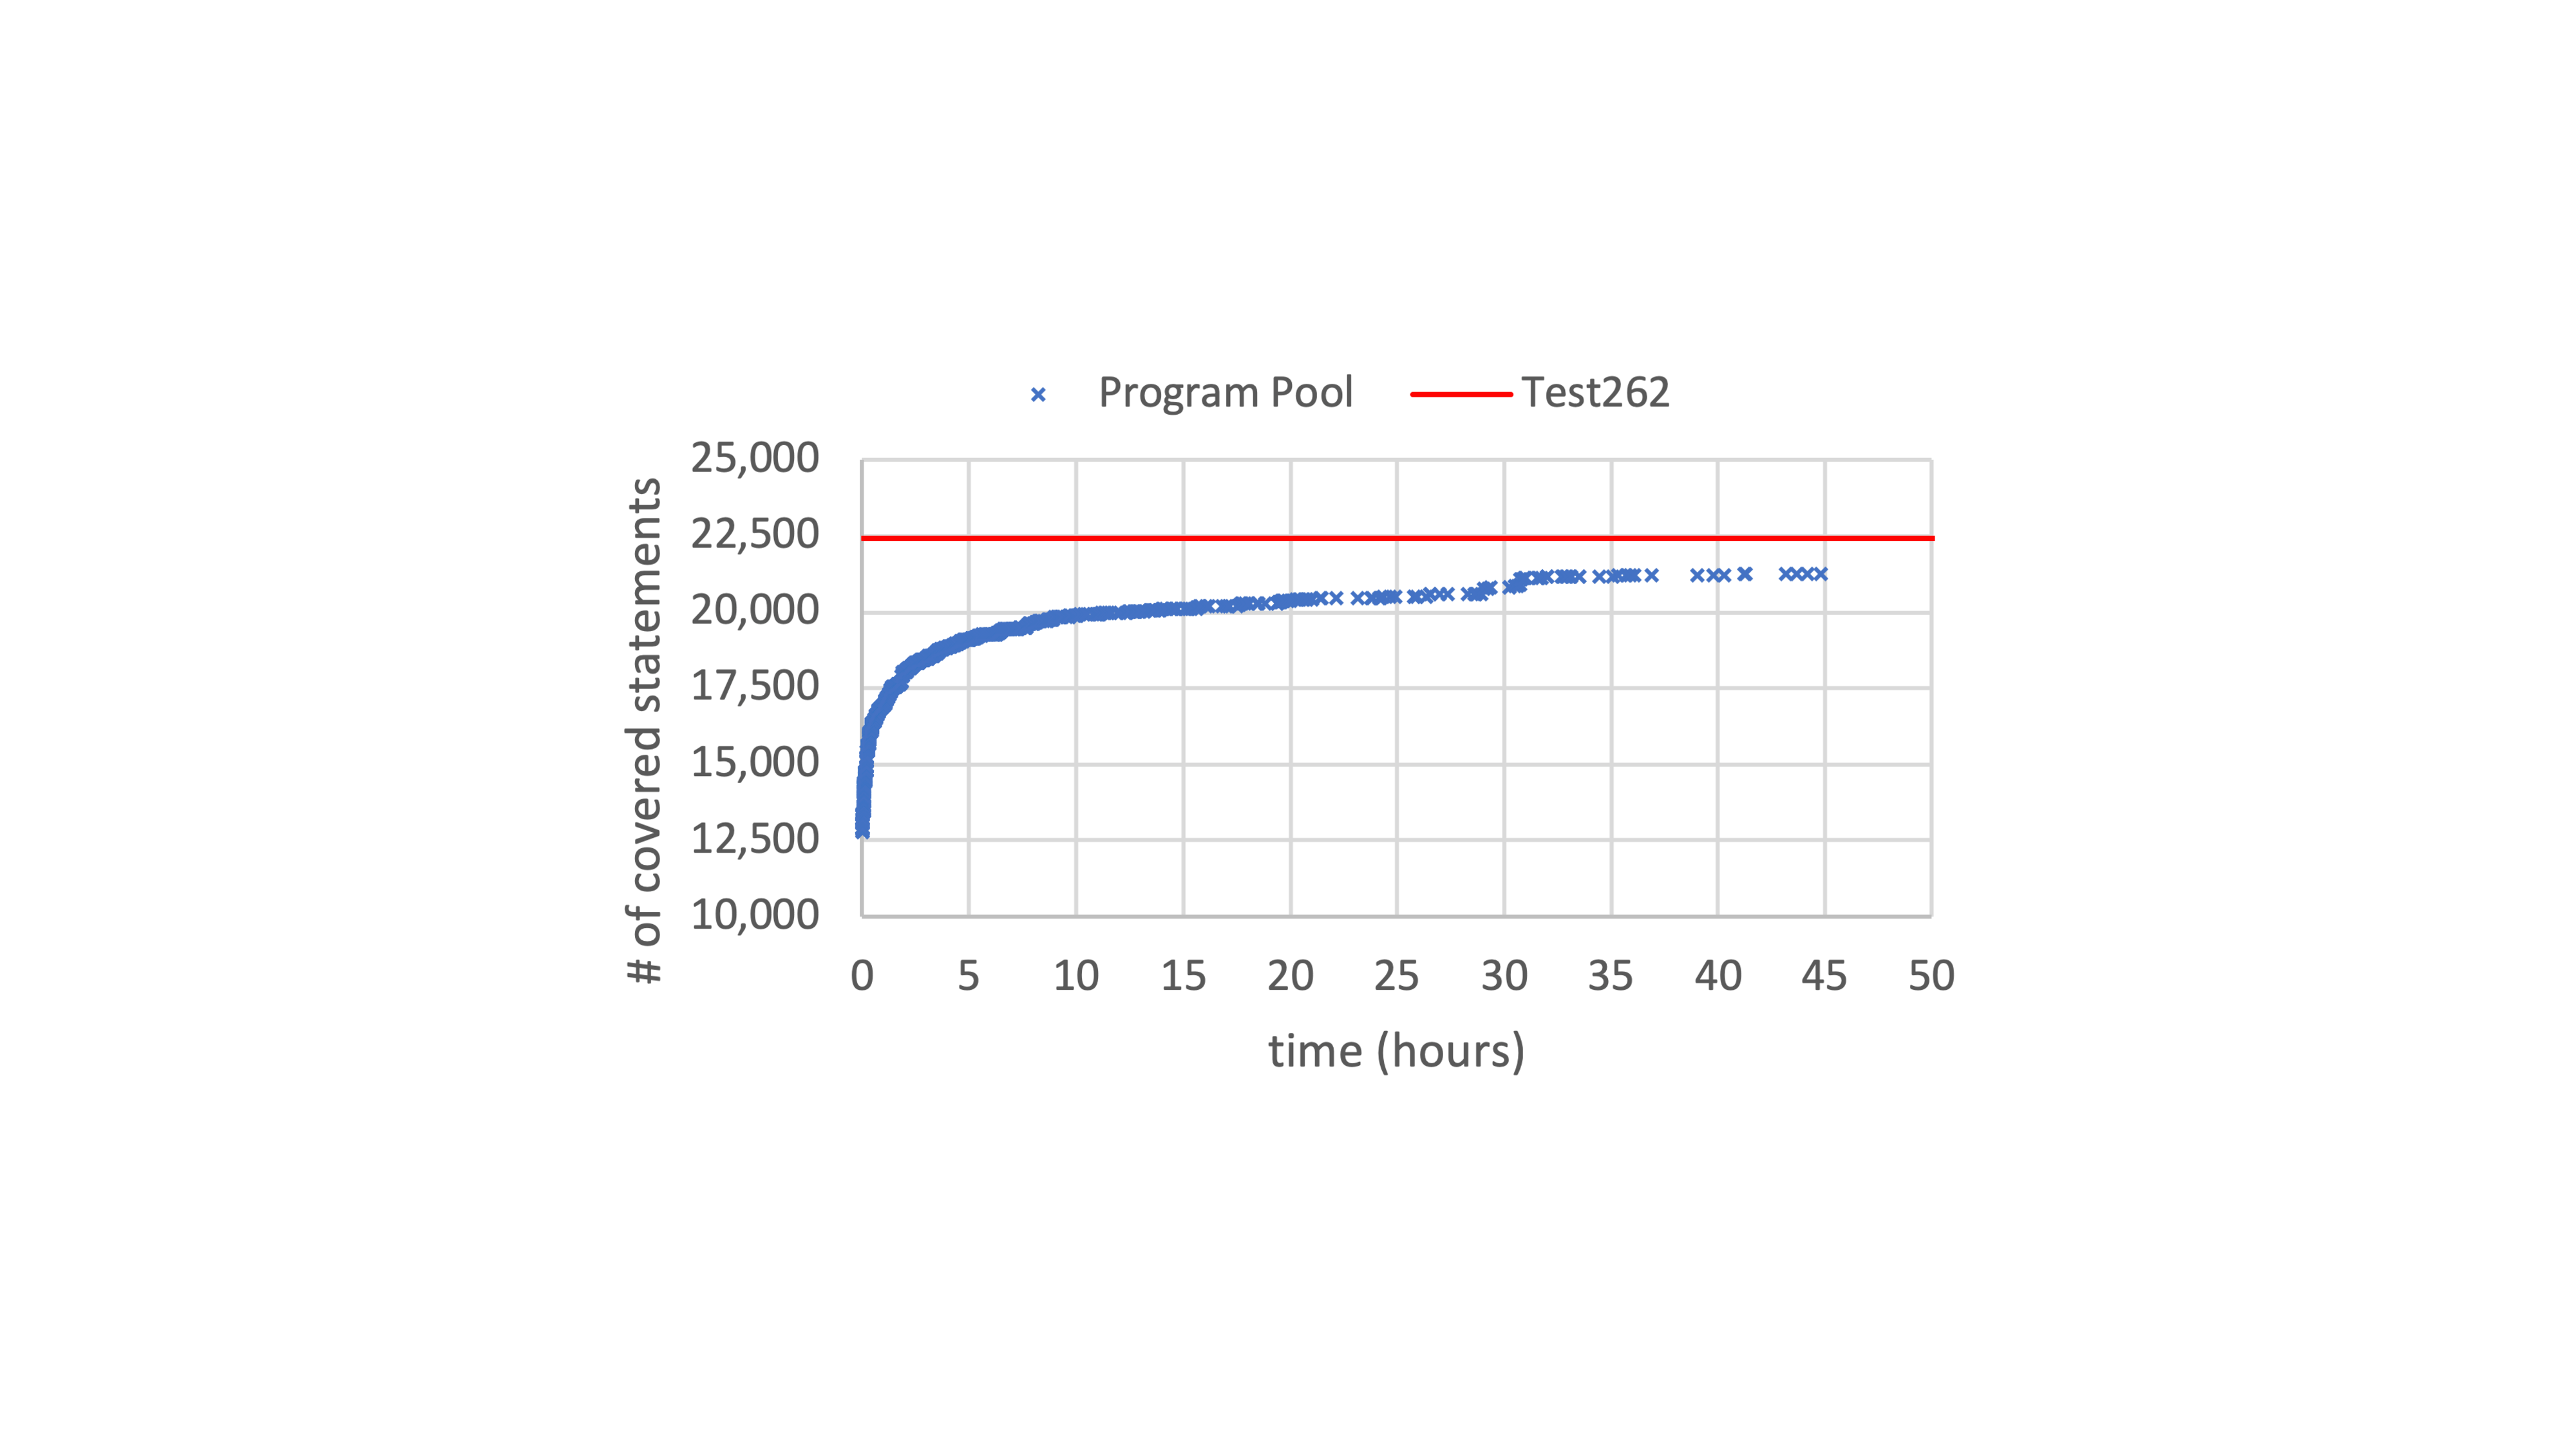
\includegraphics[width=\textwidth]{img/stmt-coverage.pdf}
    \caption{The statement coverage}
    \label{fig:stmt-coverage}
  \end{subfigure}
  \quad
  \begin{subfigure}[t]{0.48\textwidth}
    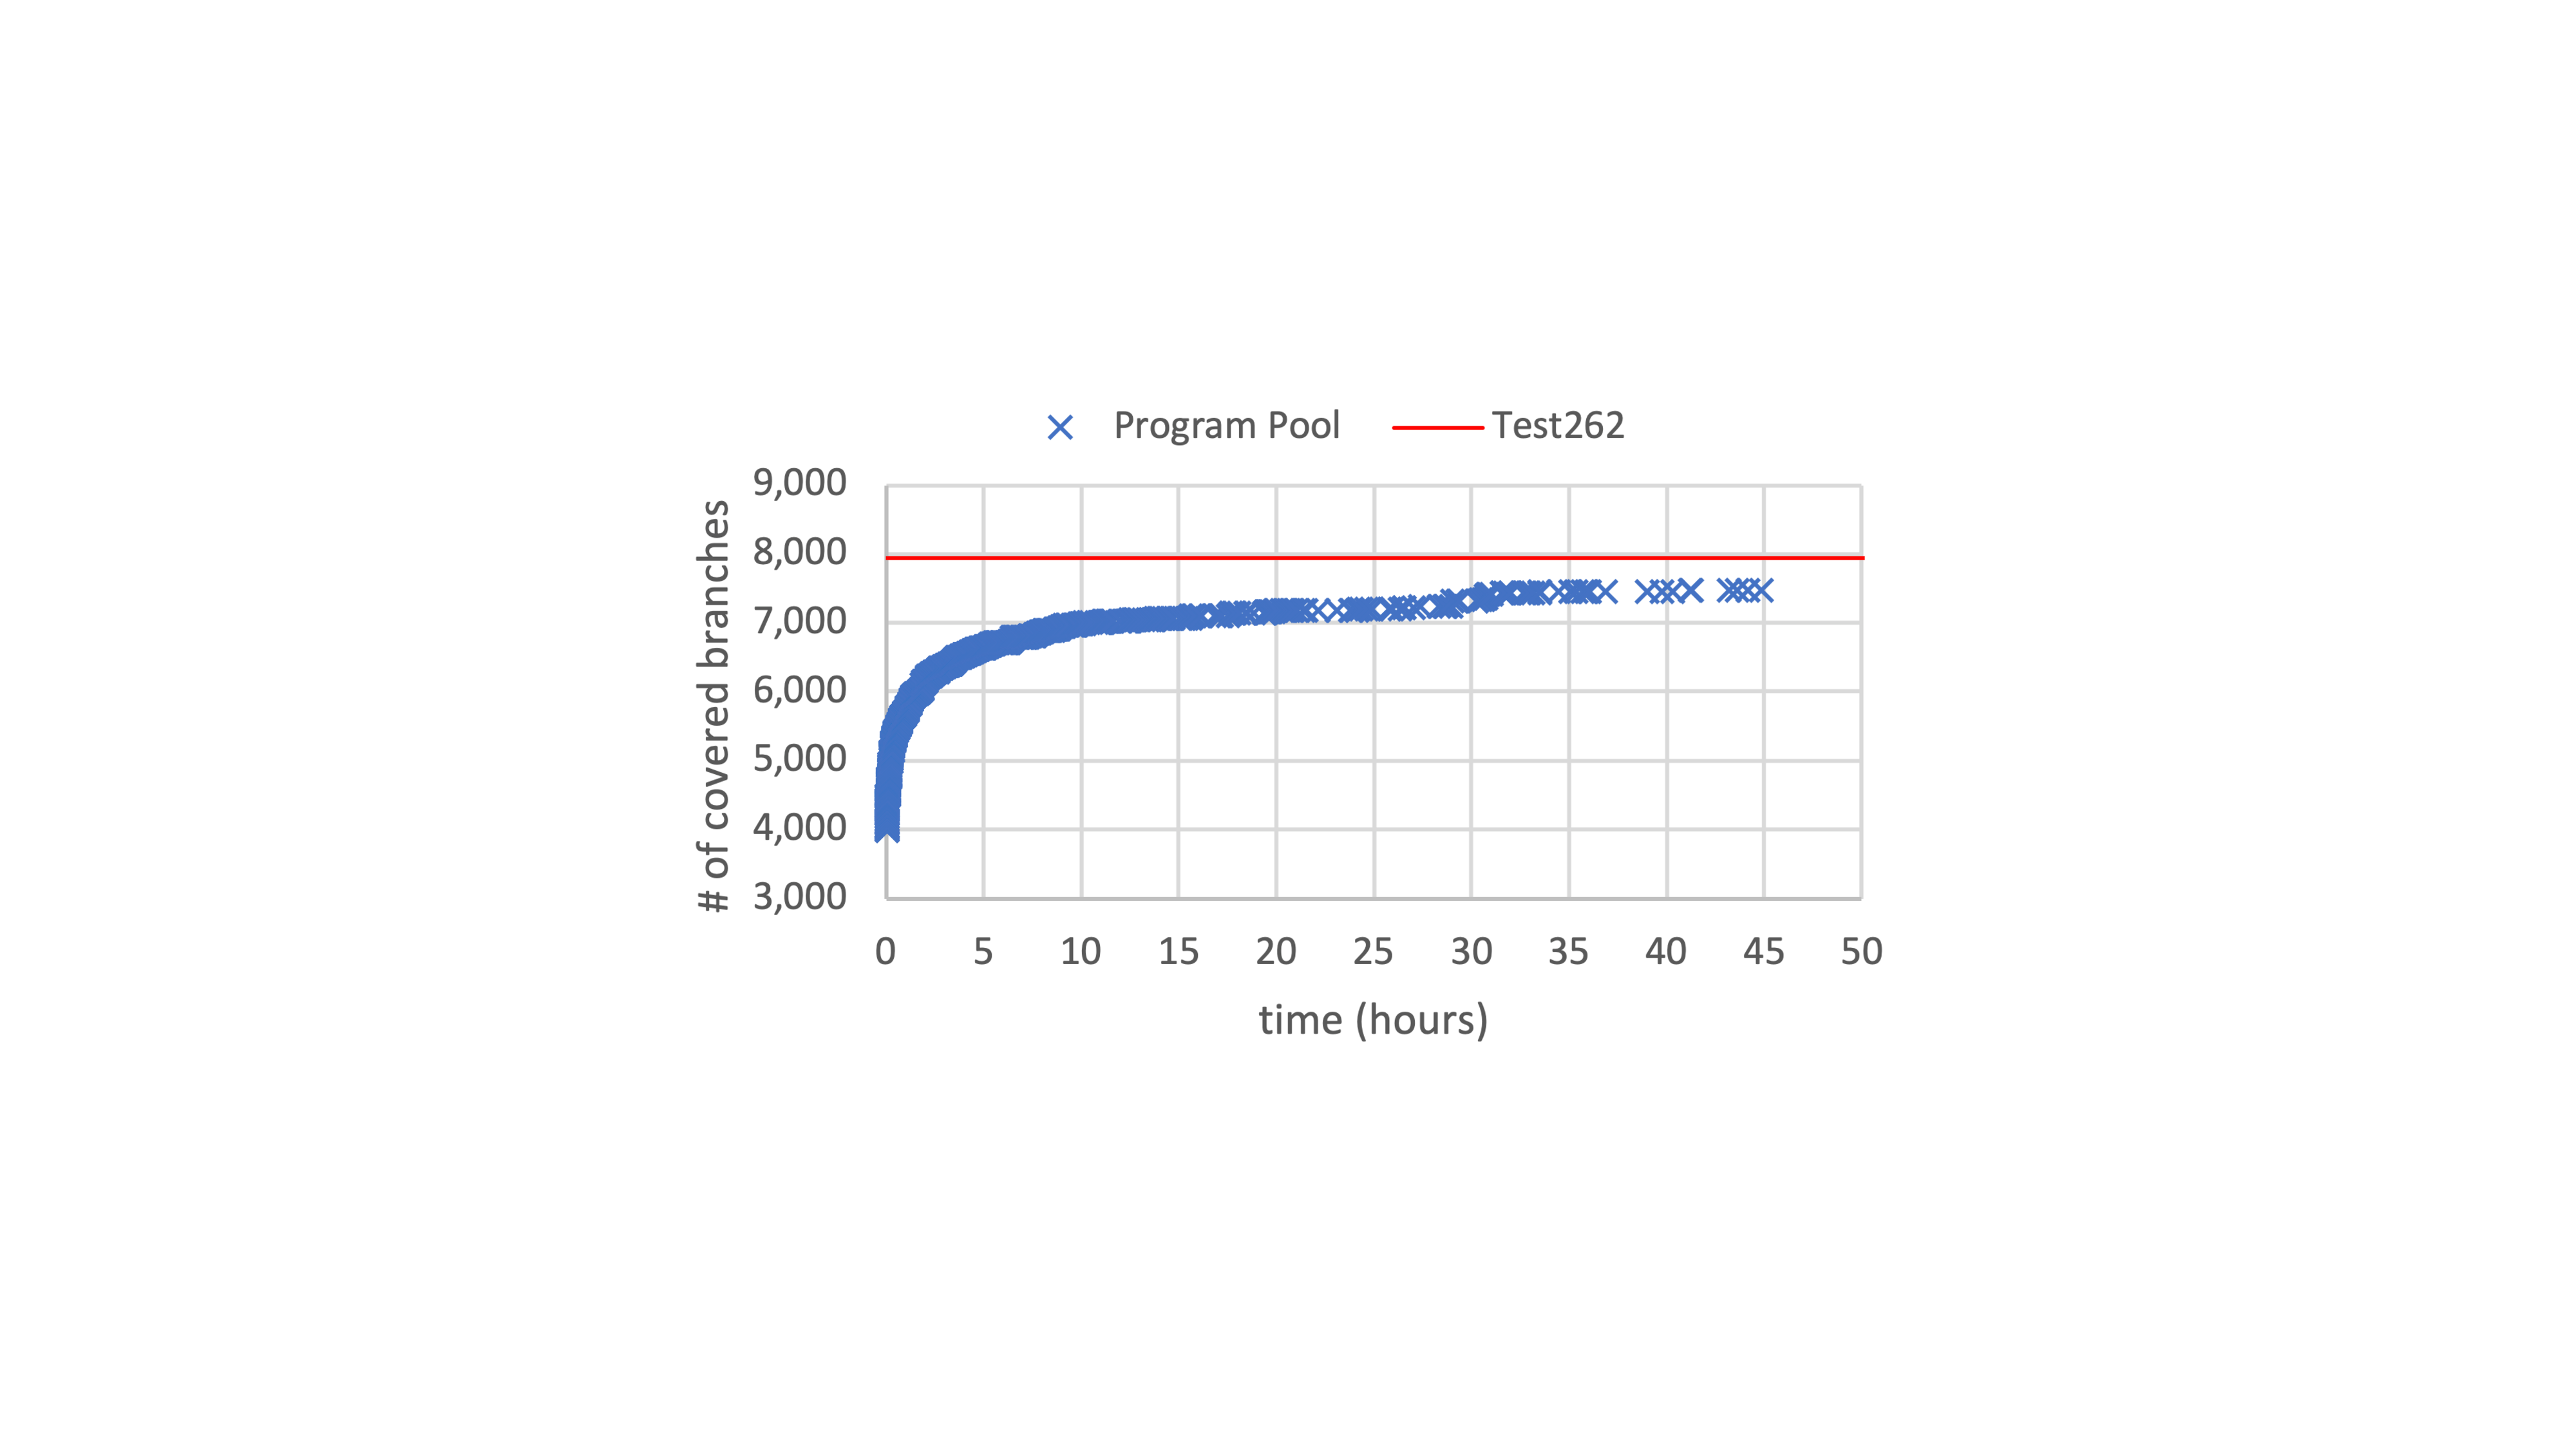
\includegraphics[width=\textwidth]{img/branch-coverage.pdf}
    \caption{The branch coverage}
    \label{fig:branch-coverage}
  \end{subfigure}
  \caption{The semantics coverage changes during the test generation phase}
  \label{fig:sem-coverage}
  \vspace*{-1em}
\end{figure*}

To evaluate $\tool$ that performs the $N$+1-version differential testing of JavaScript
engines and specification, we applied our tool to four JavaScript engines that
fully support modern JavaScript features and the most recent specification,
ECMAScript 2020 (ES11, 2020).  We targeted the following four JavaScript
engines and all of them supports
ES11\footnote{https://github.com/graalvm/graaljs\#current-status}\footnote{https://bellard.org/quickjs/}\footnote{https://blog.moddable.com/blog/xs10/}\footnote{https://v8.dev/}:
\begin{itemize}
  \item \textbf{GraalJS(v20.1.0):} A JavaScript implementation built on
    GraalVM\cite{graaljs}, which is a Java Virtual Machine (JVM) based on
    HotSpot/OpenJDK developed by Oracle.
  \item \textbf{QuickJS(2020-04-12):} A small and embedded JavaScript engine developed by
    Fabrice Bellard and Charlie Gordon\cite{qjs}.
  \item \textbf{Moddable XS(v10.2.1):} A JavaScript engine at the center of the Moddable
    SDK\cite{xs}, which is a combination of development tools and runtime
    software to create applications for micro-controllers.
  \item \textbf{V8(v8.5):} The Google's open source high-performance JavaScript and
    WebAssembly engine\cite{v8}, written in C++.
\end{itemize}
To extract mechanized specification from ECMAScript, we utilize the tool
$\jiset$, which is a JavaScript IR-based semantics extraction toolchain.
automatically extracted from a given ECMAScript.  To focus on the semantics of
core JavaScript semantics, we only consider the semantics of strict mode
JavaScript codes that pass syntax checking including the EarlyError rules.  To
filter out the JavaScript codes that are not strict or fail the syntax checking,
we utilize the syntax checker of the most reliable JavaScript engine, V8.
We performed our experiments on a machine equipped with 4.0GHz Intel(R) Core(TM)
i7-6700k and 32GB of RAM (Samsung DDR4 2133MHz 8GB*4).  We evaluated our tool
based on the following four research questions:
\begin{itemize}
  \item {\bf RQ1 (Coverage of Generated Tests)} The semantics coverage compared
    to Test262, the manually written official conformance test suite for
    ECMAScript.
  \item {\bf RQ2 (Accuracy of Bug Localization)} The accuracy of bug locations
    pointed by \mytextsf{Bug Localizer} compared to the actual bug locations.
  \item {\bf RQ3 (Bug Detection in JavaScript Engines)} The number of bugs in
    four JavaScript engines detected by $\tool$.
  \item {\bf RQ4 (Bug Detection in ECMAScript)} The number of specification bugs
    in ES11 detected by $\tool$.
\end{itemize}


\subsection{Coverage of Generated Tests}

For the first step, we synthesize seed programs via \mytextsf{Seed Synthesizer}
based on the syntax of ES11.  It synthesizes \inred{1,112} JavaScript programs
in about \inred{10} seconds and covers \inred{97.25\% (395/406)} of reachable
alternatives in syntax productions.  The seed programs becomes the initial
program pool and it gradually grows via \mytextsf{Target Selector} and
\mytextsf{Program Mutator}.  Figure~\ref{fig:sem-coverage} shows the change of
semantics coverage of the program pool during the iterative process in
\inred{50} hours.  The left and right graphs show the statement and branch
coverage, respectively.  The red line denotes the coverage of tests of Test262,
dark gray X marks denote tests generated from ES11, and blue O marks denote
tests generated from ES11 after fixing bugs detected by our tool.  For the
statement coverage, \inred{29,728} statements exist in ES11 and tests in Test262
covers \inred{22,425 (75.43\%)} statements.  The initial program pool covers
\inred{12,766 (42.94\%)} statements and the final program pool covers
\inred{21,249 (71.48\%)} and \inred{21,249 (71.48\%)} statements before and
after fixing bugs, respectively.  For branch coverage, \inred{11,448} branches
exist in ES11 and tests in Test262 covers \inred{7,944 (69.39\%)} branches.  The
initial program pool covers \inred{3,986 (34.82\%)} branches and the final
program pool covers \inred{7,476 (65.30\%)} and \inred{7,476 (65.30\%)} branches
before and after fixing bugs.

\begin{table}
  \caption{The number of successes and covered branches for mutation methods}
  \label{table:mutation-method}
  \vspace*{-1em}
  \small
  \[
    \begin{array}{l?r|r}
      \telembf{c?}{Mutation Methods}      & \telembf{c}{Success}  & \telembf{c}{Branch (Avg.)}\\\toprule\\[-1.4em]
      \text{Nearest Syntax Tree Mutation} & \rtext{436}           & \rtext{1,450 (3.33)}\\\hline
      \text{Random Mutation}              & \rtext{320}           & \rtext{910   (2.84)}\\\hline
      \text{Statement Insertion}          & \rtext{201}           & \rtext{672   (3.34)}\\\hline
      \text{Object Substitution}          & \rtext{162}           & \rtext{453   (2.80)}\\\hline
      \text{String Substitution}          & \rtext{4}             & \rtext{5     (1.25)}\\\hline
      \hline
      \telembf{c?}{Total}                 & \rtext{1,123}         & \rtext{3,490 (3.11)}\\
    \end{array}
  \]
  \vspace*{-1.5em}
\end{table}

Table~\ref{table:mutation-method} shows the number of successes and covered
branches for each mutation method during the test generation phase.  In total,
$\tool$ succeeds to synthesize \inred{1,123} programs that covers \inred{3,490}
more branches than the initial program pool.  Among five mutation methods, the
nearest syntax tree mutation is the most contributed method (\inred{436}
successes and \inred{1,450} covered branches) and the least one is the string
substitution (\inred{4} successes and \inred{5} covered branches).  On average,
\inred{3.11} branches are covered by one successful mutation.

Finally, $\tool$ generates \inred{X,XXX} JavaScript programs and the average
length of generated programs is \inred{XX.XX}.  After injecting assertions by
\mytextsf{Assertion Injector}, generated programs become conformance tests and
their average length is \inred{XXX.XX}.  Compared to Test262, the number of
generated tests are much smaller and their sizes also shorter than that of tests
in Test262.  Test262 provides \inred{XX,XXX} tests for the same range of
semantics and their average size is \inred{XXX.XX}.


\subsection{Accuracy of Bug Localization}

\begin{figure}[t]
  \centering
  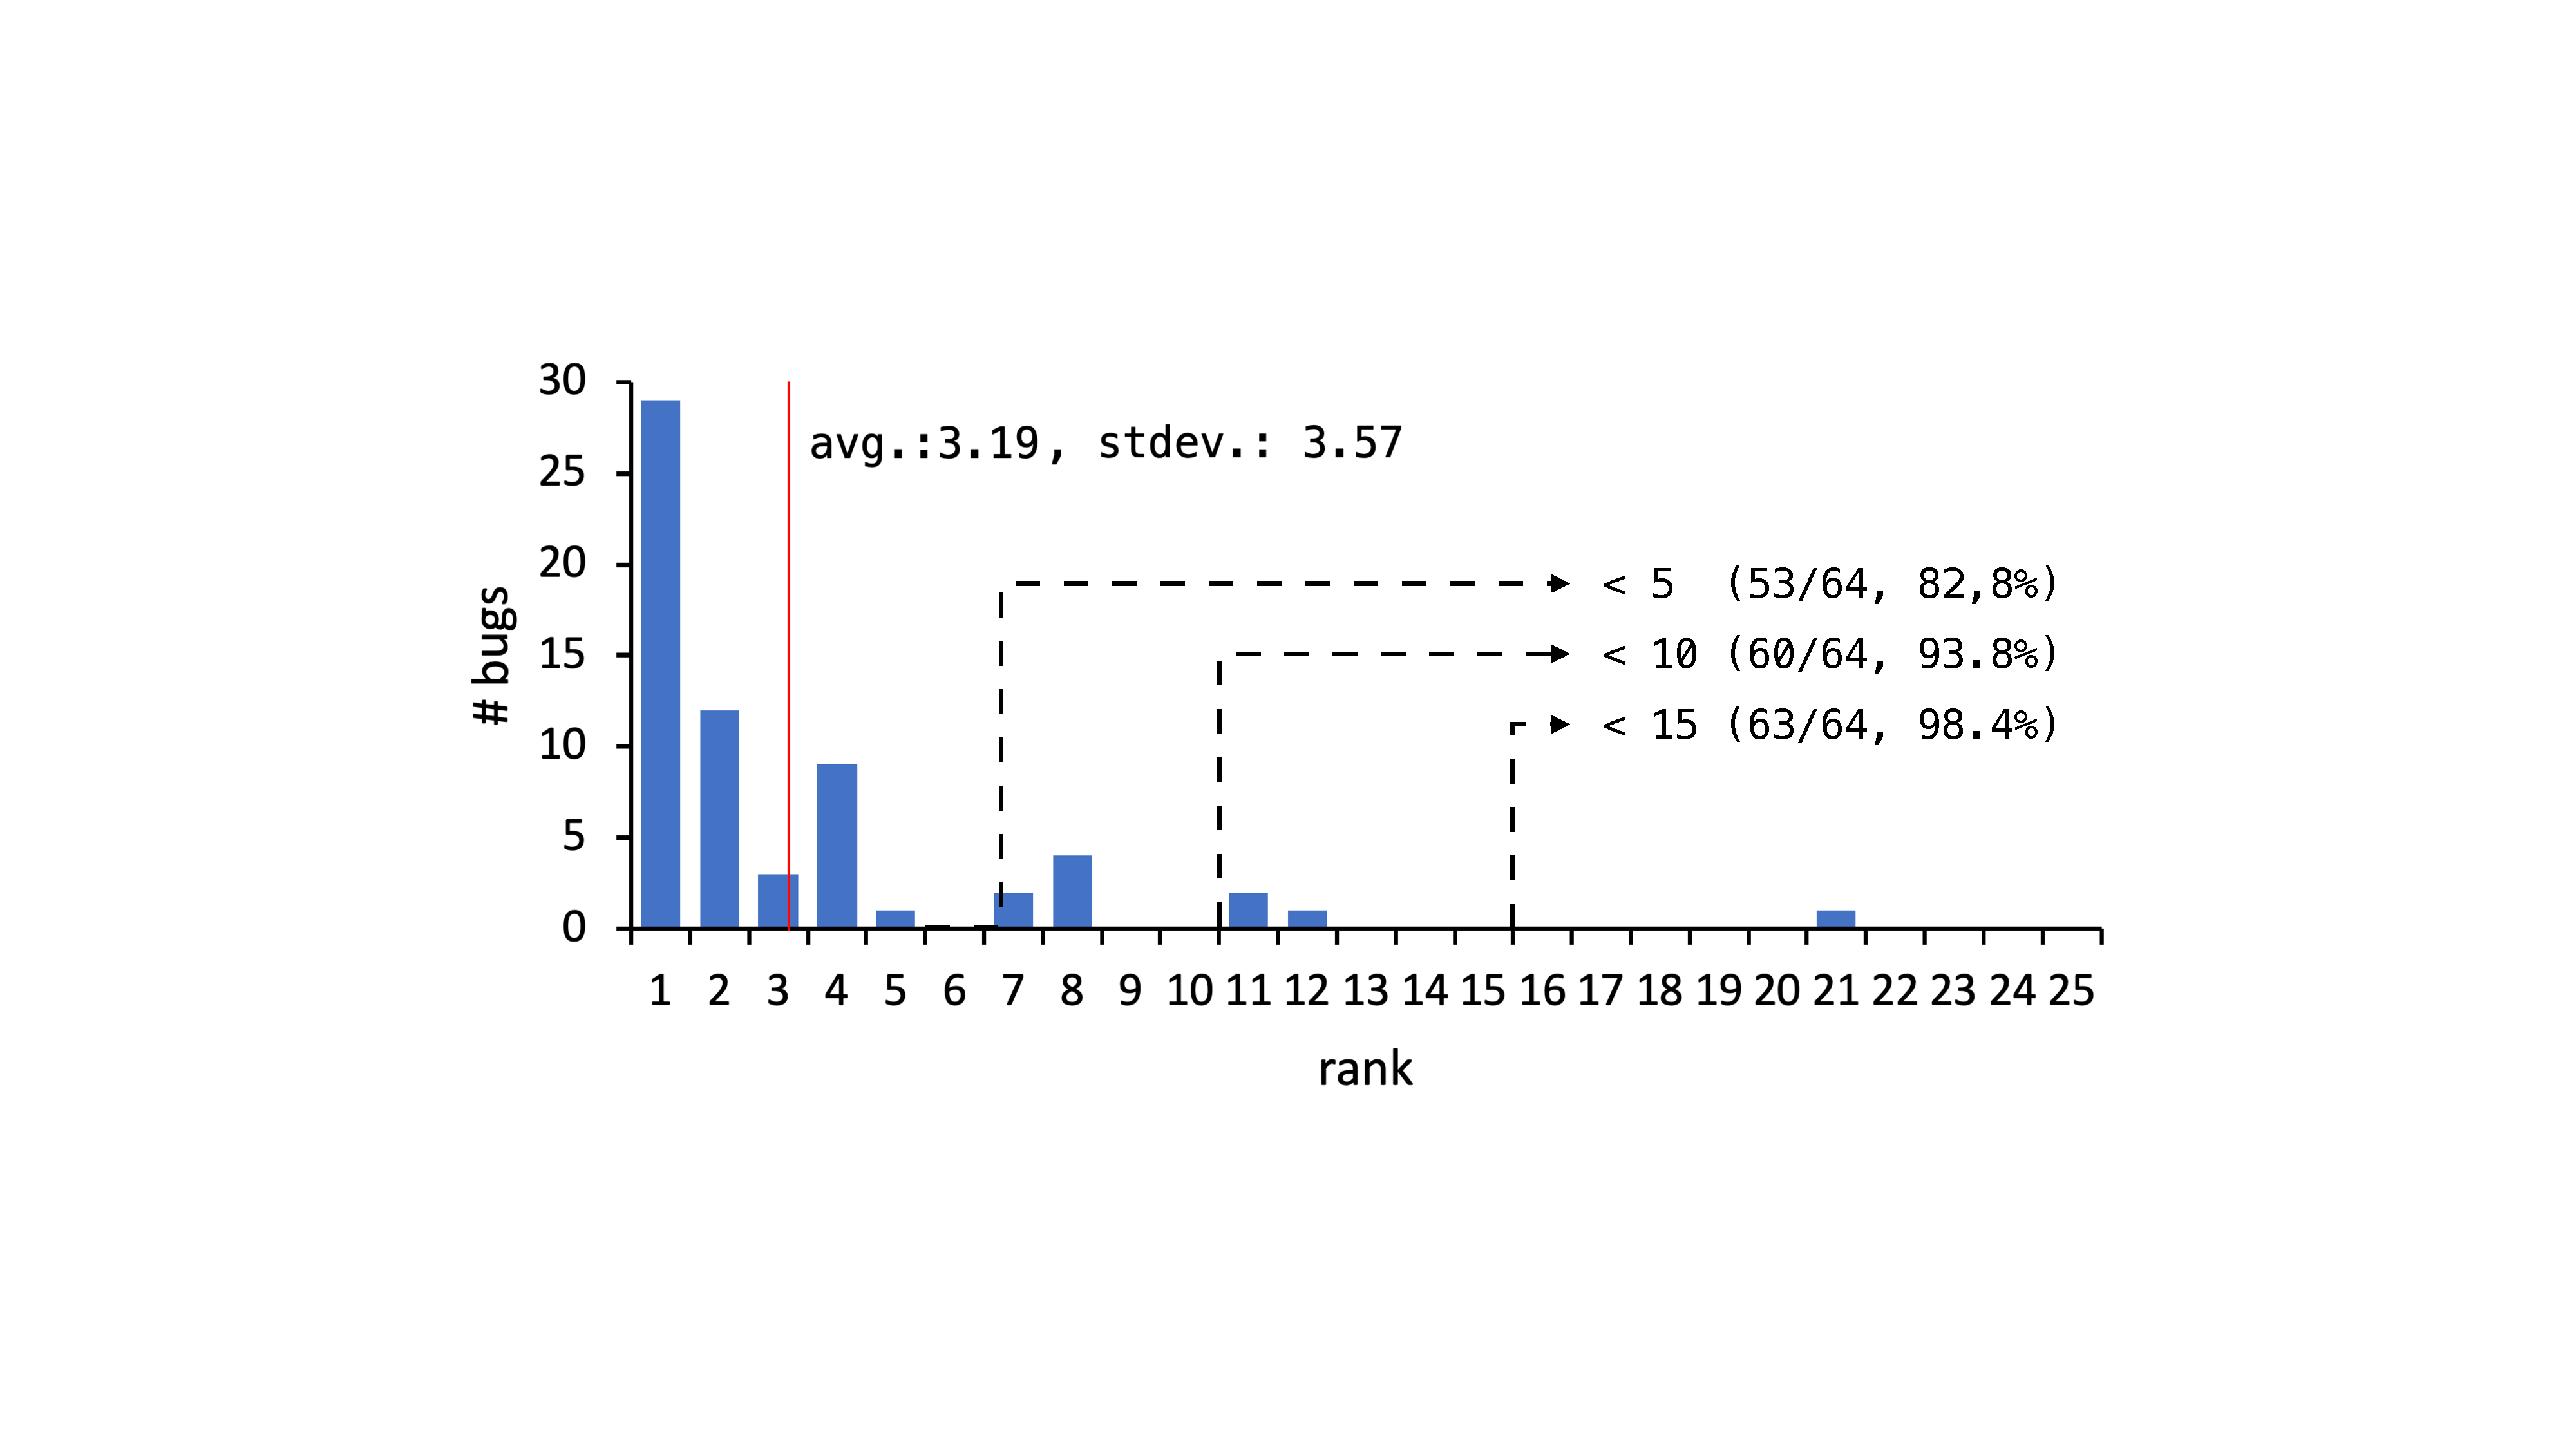
\includegraphics[width=0.48\textwidth]{img/localize.pdf}
  \caption{Ranks of actual buggy alogrithms in results of \mytextsf{Bug Localizer}
    for bugs detected by $\tool$}
  \label{fig:localize}
  \vspace*{-1em}
\end{figure}

We executed the generated conformance tests on four different JavaScript engines
to find engine or specification bugs.  We utilize the majority of execution
results to assort bugs as engine or specification bugs.  If most of engines
fails to a specific conformance test, we believe that the failure of the test
represents the correct semantics.  Thus, we suspect engines passing the test and
the specification of containing bugs related to the test.  Otherwise, we assume
that bugs exist in engines failing the test.  We manually checked the detected
bugs whether they are actually engine bugs or specification bugs.  The following
table shows the number of engines failing tests related to each bug.

\begin{table}[H]
  \centering
  \vspace*{-1em}
  \small
  \[
    \begin{array}{l?r|r|r|r?r?r}
      \telembf{c?}{\# Fails} &
      \telembf{c}{1} &
      \telembf{c}{2} &
      \telembf{c}{3} &
      \telembf{c?}{4} &
      \telembf{c?}{Total} &
      \telembf{c}{Avg.} \\\toprule\\[-1.4em]

      \text{Engine Bugs}  & \inred{-} & \inred{-} & \inred{-} & \inred{-} & \inred{39} & \inred{1.3}\\\hline
      \text{Spec. Bugs}   & \inred{-} & \inred{-} & \inred{-} & \inred{-} & \inred{7} & \inred{3.8}
    \end{array}
  \]
  \vspace*{-1em}
\end{table}

According to the table, our assumption seems to be reliable because tests
related to engine bugs failed in \inred{1.3} engines on average.  For
specification bugs, the related tests failed in \inred{3.8} engines on average.

Based on results of conformance tests on four JavaScript engines, we localize
the specification or engine bugs on the semantics of ES11.  We detected
\inred{-} bugs and Figure~\ref{fig:localize} shows the ranks of their actual
buggy algorithms in results of \mytextsf{Bug Localizer}.  The average rank is
\inred{-}, and \inred{-}\% of buggy algorithms are ranked in less than 5,
\inred{-}\% in less than 10, and \inred{-}\% in less than 15.  Among \inred{-}
bugs, locations of \inred{-} bugs are ranked in more than \inred{-}.  It shows
the limitation of the statistical fault localization that have low accuracy of
localization for bugs caused by missing statements.  For example, \inred{TODO:
example}.



\subsection{Bug Detection in JavaScript Engines}

\begin{table}
  \caption{The number of engine bugs detected by $\tool$}
  \label{table:engine-bug}
  \vspace*{-1em}
  \small
  \[
    \begin{array}{l?r|r|r|r|r|r|r?r}
      \telembf{@{}c@{~}?}{Engines} &
      \telemsf{@{~}c@{~}|}{Exc} &
      \telemsf{@{~}c@{~}|}{Crash} &
      \telemsf{@{~}c@{~}|}{Var} &
      \telemsf{@{~}c@{~}|}{Obj} &
      \telemsf{@{~}c@{~}|}{Desc} &
      \telemsf{@{~}c@{~}|}{Key} &
      \telemsf{@{~}c@{~}?}{In} &
      \telembf{@{~}c@{}}{Total}\\\toprule\\[-1.4em]

      \text{GraalJS}      & \inred{-} & \inred{-} & \inred{-} & \inred{-} & \inred{-} & \inred{-} & \inred{-} & \inred{10}\\\hline
      \text{QuickJS}      & \inred{-} & \inred{-} & \inred{-} & \inred{-} & \inred{-} & \inred{-} & \inred{-} & \inred{6}\\\hline
      \text{Moddable XS}  & \inred{-} & \inred{-} & \inred{-} & \inred{-} & \inred{-} & \inred{-} & \inred{-} & \inred{21}\\\hline
      \text{V8}           & \inred{-} & \inred{-} & \inred{-} & \inred{-} & \inred{-} & \inred{-} & \inred{-} & \inred{2}\\\hline
      \hline
      \telembf{c?}{Total} & \inred{-} & \inred{-} & \inred{-} & \inred{-} & \inred{-} & \inred{-} & \inred{-} & \inred{39}
    \end{array}
  \]
  \vspace*{-1.5em}
\end{table}

Based on the above approach, our tool detected \inred{39} engine bugs on four
different JavaScript engines: \inred{-} for GraalJS, \inred{-} for QuickJS,
\inred{-} for Moddable XS, and \inred{-} for V8.  Table~\ref{table:engine-bug}
shows the number of detected bugs for each engine and depending on used
assertions.  We injected seven different kinds of assertions for exceptions
(\mytextsf{Exc}), crashes (\mytextsf{Crash}), variable values (\mytextsf{Var}), object
values (\mytextsf{Obj}), property descriptors (\mytextsf{Desc}), property keys
(\mytextsf{Key}), and internal methods and slots (\mytextsf{In}).  For bug
detection, usefulness of each assertion is different with each other.  The
assertions \mytextsf{Exc} and \mytextsf{Key} are top-two to detect engine bugs and
they detects \inred{-} and \inred{-} bugs out of \inred{39} bugs, respectively.
\inred{The \mytextsf{Var} detects - engine bugs but other assertions failed to
detect engine bugs.}

The most reliable JavaScript engine is V8 because it contains only two bugs and
they are caused by specification bugs in ES11.  V8 strictly follows the
semantics of functions described in ES11 related to the specification bugs
ES11-1 and ES11-2 listed in Table~\ref{table:spec-bug}.  Unfortunately, the
semantics is not intention of TC39 thus V8 confirmed and fixed two bugs.

The worst one is Moddable XS with \inred{-} bugs and they are located in various
language features such as optional chains, \code{Number.prototype.toString},
iterators of \code{Map}/\code{Set}, complex assignment patterns, etc.  Among
them, a bug related to optional chains shows that our approach is applicable for
new language features because optional chains are first introduced in ES11.
For example, \code{undefined?.()} should return \code{undefined} according to
the semantics of ES11 but Moddable XS throws \code{TypeError}.

We detected \inred{-} engine bugs in GraalJS and one of them raises an engine
crash.  When we apply the prefix increment operator for \code{undefined},
GraalJS throws a \code{java.lang.IllegalStateException}.  Moreover, we cannot
catch this exception using \code{try} statements:
\begin{lstlisting}[style=myJSstyle]
try { ++undefined; } catch(e) { }
\end{lstlisting}
The authors of GraalJS were interesting to our work because conformance tests
generated by our tool detected many semantics bugs that cannot be detected by
other conformance tests.  Moreover, they claimed that they want to use our
conformance tests in the continuous integration (CI) progress of GraalJS.

QuickJS have \inred{-} engine bugs most of them related to the corner cases of
semantics of functions.  For example,
\begin{lstlisting}[style=myJSstyle]
function f (... { x = x }) { return x; } f()
\end{lstlisting}
it should throw a \code{ReferenceError} because the variable \code{x} is not yet
initialized when the program tries to read the right-hand side of \code{x = x}
in the object assignment pattern.  However, QuickJS assumes that the initial
value of the variable \code{x} is \code{undefined} thus the function call
\code{f()} returns \code{undefined}.


\subsection{Bug Detection in ECMAScript}

\begin{table*}[t]
  \centering
  \caption{Specification bugs in ECMAScript 2020 (ES11) detected by $\tool$}
  \label{table:spec-bug}
  \vspace*{-.5em}
  \small
  \begin{tabular}{@{}c@{~}?c|@{~}c@{~}|l|c|c|@{~}c@{~}|@{~}c@{~}|@{~}r@{}}
    \telembf{@{}c?}{\bf Name} &
    \telembf{c}{\bf Feature} &
    \telembf{@{}c@{~}}{\bf \#} &
    \telembf{c}{\bf Description} &
    \telembf{@{~}c@{~}}{\bf Assertion} &
    \telembf{@{~}c}{\bf Known} &
    \telembf{@{}c}{\bf Created} &
    \telembf{@{}c}{\bf Resolved} &
    \telembf{@{}c@{~}}{\bf Existed} \\\toprule\\[-1.4em]

    ES11-1 &
    \text{Function} &
    \inred{-} &
    \makecell[l]{Wrong order between property keys for functions} &
    \mytextsf{Key} &
    O &
    2019-02-07 &
    2020-04-11 &
    429 days \\\hline

    ES11-2 &
    \text{Function} &
    \inred{-} &
    \makecell[l]{Missing property \code{name} for anonymous functions} &
    \mytextsf{Key} &
    O &
    2015-06-01 &
    2020-04-11 &
    1,776 days \\\hline

    ES11-3 &
    \text{Loop} &
    1 &
    \makecell[l]{Returning iterator objects instead of iterator records\\
      in \textbf{ForIn/OfHeadEvaluation} for \code{for-in} loops} &
    \mytextsf{Exc} &
    O &
    2017-10-17 &
    2020-04-30 &
    926 days \\\hline

    ES11-4 &
    \text{Expression} &
    4 &
    \makecell[l]{Using the wrong variable \code{oldvalue} instead of\\
      \code{oldValue} in \textbf{Evaluation} of \textit{UpdateExpression}} &
    \mytextsf{-} &
    O &
    2019-09-27 &
    2020-04-23 &
    209 days \\\hline

    ES11-5 &
    \text{Expression} &
    1 &
    \makecell[l]{Unhandling abrupt completion\\
      in \textbf{Abstract Equality Comparison}} &
    \mytextsf{Exc} &
    O &
    2015-06-01 &
    2020-04-28 &
    1,793 days \\\hline

    ES11-6 &
    \text{Object} &
    1 &
    \makecell[l]{Unhandling abrupt completion in \textbf{Evaluation} of\\
      \textit{PropertyDefinition} for object literals} &
    \mytextsf{Exc} &
    X &
    2019-02-07 &
    \inred{-} &
    \inred{-} days

    % ES11-X &
    % \inred{\text{-}} &
    % \makecell[l]{-} &
    % \inred{\mytextsf{???}} &
    % \inred{-} &
    % \inred{-} &
    % \inred{-} &
    % \inred{-} days
  \end{tabular}
\end{table*}

Our tool detected not only engine bugs but also \inred{-} specification bugs in
ES11, the most recent version of ECMAScript. We categorized them based on their
root causes from ES11-1 to ES11-7 in Table~\ref{table:spec-bug}.  Among them,
six categories (ES11-1 to ES11-6) were already reported and fixed in the current
draft of the next ECMAScript but the remaining one, ES11-7, was never reported
before.  We reported the bug ES11-7 and TC39 confirmed that it is an actual
specification bug.  Thus, it will be fixed in the next version, ECMAScript 2021
(ES12).  Now, we explain the details of specification bugs our tool detected.

ES11-1 contains \inred{-} specification bugs are due to a wrong order between
property keys of all kinds of function values such as \code{async}/generator
functions, arrow functions, or classes.  For example, if we define a class
declaration with a name \code{A} (\code{class A {}}), three properties are
defined in the function stored in the variable \code{A}: \code{length} with a
number value \code{0}, \code{prototype} with an object, and \code{name} with a
string \code{"A"}.  The problem is the different order of their keys because of
the wrong order of their creations.  From ECMAScript 2015 (ES6), the order
between property keys is no more implementation-dependent feature and it is
related to the creation order of properties.  According to the semantics of
ES11, the order of property keys in the class \code{A} should be \code{[length,
prototype, name]} but three engines except V8 claims that \code{[length, name,
prototype]}.  In fact, the three engines are correct thus the ES11 and V8
confirmed that it is a real bug.  This bug was created on \inred{-} and TC39
fixed it on \inred{-} after \inred{-} days.

Similarly, ES11-2 contains \inred{-} specification bugs related to all kinds of
anonymous functions.  Until ES10, anonymous functions, such as an identity arrow
function \code{x => x}, have their own property \code{name} with an empty string
\code{""}.  However, ES11 removes the \code{name} property but still three
engines except V8 creates the \code{name} property in anonymous functions.  In
fact, the removal was not intention of TC39 and it was reverted to create the
property again on \inred{-}.  Moreover, V8 also accepted that it was the engine
bug and it will be fixed in V8.

The bug in ES11-3 comes from the misunderstanding of the term ``iterator
object'' and ``iterator record''.  The algorithm \textbf{ForIn/OfHeadEvaluation}
should return an iterator record, which is an implicit record consists of only
internal slots.  However, In ES11, it returns an iterator object, which is a
JavaScript object with some properties related to iterations.  It causes a
\code{TypeError} when executing the code \code{for(var x in \{\});} according to
ES11 but all engines normally execute the code without any exceptions.  This bug
is confirmed by TC39 on \inred{-}.

ES11-4 contains four specification bugs caused by a typo for the variable in the
semantics of four different update expressions (\code{x++}, \code{x--},
\code{++x}, and \code{--x}).  In each \textbf{Evaluation} of four kinds of
\textit{UpdateExpression}, there exists a typo \code{oldvalue} in the step 3
instead of \code{oldValue} declared in the step 2.  Our tool failed to execute
the code \code{x++} using the semantics of ES11 because of the typo.  In this
case, we directly pass the code to \mytextsf{Bug Localizer} to test whether the
code is executable in real engines and to localize the bug.  Of course, four
JavaScript engines succeed to execute the update expressions without any issues
and this bug was confirmed by TC39 on \inred{-}.

Two bugs in ES11-5 and ES11-6 are caused by unhandling of abrupt completions in
the abstract equality comparison and property definitions of object literals,
respectively.  While the bug in ES11-5 confirmed by TC39 and was fixed on
\inred{-}, the bug in ES11-7 was not yet discovered thus we reported it and
confirmed by TC39 on \inred{-} after existing for \inred{-} days.

\section{Related Work}\label{sec:related}
\inred{TODO}

\begin{itemize}
  \item CodeAlchemist\cite{codealchemist}
  \item Csmith\cite{csmith}
  \item Grammar-based Whitebox Fuzzing\cite{grammar-whitebox}
  \item Montage\cite{montage}
  \item QuickCheck\cite{quickcheck}
  \item SAGE\cite{sage}
  \item Rnadom String from a CFG\cite{cfg-gen}
  \item differential Testing for Lifter\cite{ir-diff-test}
  \item NEZHA\cite{nezha}
  \item JavaScript History\cite{js-hopl}
  \item JISET\cite{jiset}

\end{itemize}

\section{Conclusion}\label{sec:conclude}
\inred{TODO}


\normalem
\bibliographystyle{ACM-Reference-Format}
\bibliography{ref}

\end{document}
